%\chapter{U--\protect\NoCaseChange{Mo} fuel: a brief introduction}
\chapter{Introduction}
Since the discovery of fission in 1938, the world has experienced the impact of nuclear power on modern society. The primary fuel for fission is $^{235}$U\@. Naturally-occurring uranium consists of a combination of different isotopes: about 99.3\% $^{238}$U (wt\%),  0.7\% $^{235}$U, and trace amounts of $^{234}$U\@. Uranium can be ``enriched'' in the $^{235}$U isotope by using various complicated processes that mainly use the difference in mass and other physical properties. A typical power generating reactor requires less than 5\% uranium enrichment. Research reactors which require higher neutron fluxes, need a higher percentage of uranium enrichment. The neutron produced by a research reactor can be used for neutron scattering, testing and analysis of materials, production of radioisotopes, and training. Research and test reactors are also referred as non-power reactors.
The enrichment, or weight fraction of $^{235}$U, specifies the key factors of any uranium content, both in terms of research reactor fuel performance and in nuclear weapons. Above a certain enrichment, the fissile material can be turned into explosive devices. As a result, low-enriched uranium (LEU) and high-enriched uranium (HEU) have been introduced. Historically, this limit has been set at an enrichment of 20\%~\cite{glaser2005enrichment, international2005iaea}.

%After the Manhattan project, highly enriched uranium ($>$ 90\% $^{235}$U) has been used peaceful in scientific research and radioisotope production. Nuclear fuels are characterized by a unique combination of physics, engineering, safety requirements, social and environmental factors, and international concerns. The purpose of nuclear safety is to prohibit the uncontrolled release of the radioactive isotopes to the environment and ensuring safe use of fissile material. Highly enriched uranium (HEU) fuel is also a proliferation concern. All enrichments above 20\% $^{235}$U are considered HEU~\cite{glaser2005enrichment, international2005iaea}.
Using HEU in research reactors leads to a series of unavoidable and apparent proliferation\footnote{``proliferation'' in the context of nuclear energy is defined as ``the spread of nuclear weapons and technologies and the materials to make them''~\cite{montgomery2009}.} risks that are related to diversion and theft of the fissile material~\cite{donnelly1980}.
HEU can be used to make nuclear explosives, such as the one used on Hiroshima by the United States in World War II. That weapon, code named ``Little Boy,'' contained about 50 kilograms of $^{235}$U with an average enrichment of about 80\%~\cite{serber1992alamos}. The neutron production in 60 kg of metallic enriched uranium (from both fission and (\textalpha, n) reactions on oxygen) is about 100 per second. This production rate and combined with a neutron reflector can be made into a highly-enriched uranium weapon. Although there is disagreement about the likelihood of a rogue nation acquiring the necessary technical capabilities to make a nuclear weapon with an implosion design, there is little argument that it is much easier to design a so-called gun-type weapon that could work without being tested.

Proliferation concerns about HEU resulted in a global effort, led by the USA, to eliminate civilian uses of HEU in research and test reactors. One of the important HEU reduction programs is known as the Reduced Enrichment for Research and Test Reactors (RERTR) program. The RERTR program was initiated in the USA in the late 1970s to develop new nuclear fuels to replace high-enriched uranium (HEU)~\cite{travelli1980current,snelgrove1997development}\@.  The RERTR program is now managed by the U. S. National Nuclear Security Administration's (NNSA) Office of Material Management and Minimization~\cite{burkes2021thermal}. The development of low-enrichment uranium (LEU) fuels for high-performance reactors is an important nonproliferation initiative.

The RERTR initiative has completed a total of 69 reactor conversions to use LEU fuel, and 26 HEU-based reactor facilities have been verified to have been shut down~\cite{wilson2017us}. The conversion of six domestic high-performance research reactors\footnote{The Advance Test Reactor (ATR) at Idaho National Laboratory (INL), Idaho; the Advanced Test Reactor Critical (ATRC) Assembly at INL, Idaho; the High Flux Isotope Reactor (HFIR) at Oak Ridge National Laboratory (ORNL), Tennessee;  the Massachusetts Institute of Technology Reactor (MITR), Massachusetts; the National Bureau of Standards Reactor (NBSR) in Gaithersburg, Maryland; and the University of Missouri Research Reactor (MURR) in Columbia, Missouri.} that still use high-enriched uranium fuel is yet to be achieved. Due to their unique operating conditions, converting these six reactors will not be easy, and a plethora of nuclear engineering challenges are associated with their conversion. These conversion processes may take longer time periods, but developing a new LEU fuel is essential to ensure better performance and while limiting nuclear proliferation. The timeline for the conversion is currently estimated to be 10--16 years~\cite{national2016reducing, national2012progress, kaufmann1962nuclear}. 


Research reactors operate at relatively low peak fuel temperatures, but they are required to meet fuel performance requirements at high burnup. A typical peak fuel centerline temperature in a research reactor is around 250\textdegree C~\cite{meyer2014irradiation}. For a research reactor, fission densities are usually in the range of $3\times10^{21}$ to $6\times10^{21}$ fissions/cm$^3$. In some cases, peak fuel fission density exceeds $7\times10^{21}$ fissions/cm$^3$, requiring a higher density of $^{235}$U atoms. Consequently, one of the main requirements of LEU fuels is increased uranium density, such as that found in metallic uranium, to offset the decrease in \textsuperscript{235}U enrichment. 

\section{Metallic Uranium and Alloys}
Uranium, an actinide, has three allotropic forms at atmospheric pressure:
$$
\ce{\text{\textalpha} ->[$662\text{\textdegree C}$] $\text{\textbeta}$ ->[$774\text{\textdegree C}$] $\text{\textgamma}$ }
$$
The orthorhombic (\textalpha-phase), stable from below room temperature to 662\textdegree C; tetragonal (\textbeta-phase), stable from 662 to 774\textdegree C; and body-centered cubic (\textgamma-phase), stable from 772\textdegree C to the melting point, 1132~\textdegree C~\cite{kaufmann1962nuclear}. Metallic uranium at standard temperature is thought to have sufficient density ($19.05\pm0.02$ g/cm$^3$)\@. \textalpha-Uranium belongs to the orthorhombic system, in which the three axes are mutually perpendicular ($\vb{a}\perp \vb{b}\perp \vb{c}$) but are unequal length ($a\ne b\ne c$) (Fig.~\ref{fig_alphu})\@. This orientation of crystal is considered \textit{anisotropic}. A great deal of work has gone into studying the properties of \textalpha-uranium. Different heat treatment, corrosion, grain size analysis, mechanical and elastic property studies, and post irradiation analysis indicate that \textalpha-uranium is a poor candidate to be considered as a nuclear fuel~\cite{pugh1961swelling, loomis1962swelling, chiswik1958osti}.

\begin{figure}
\centering
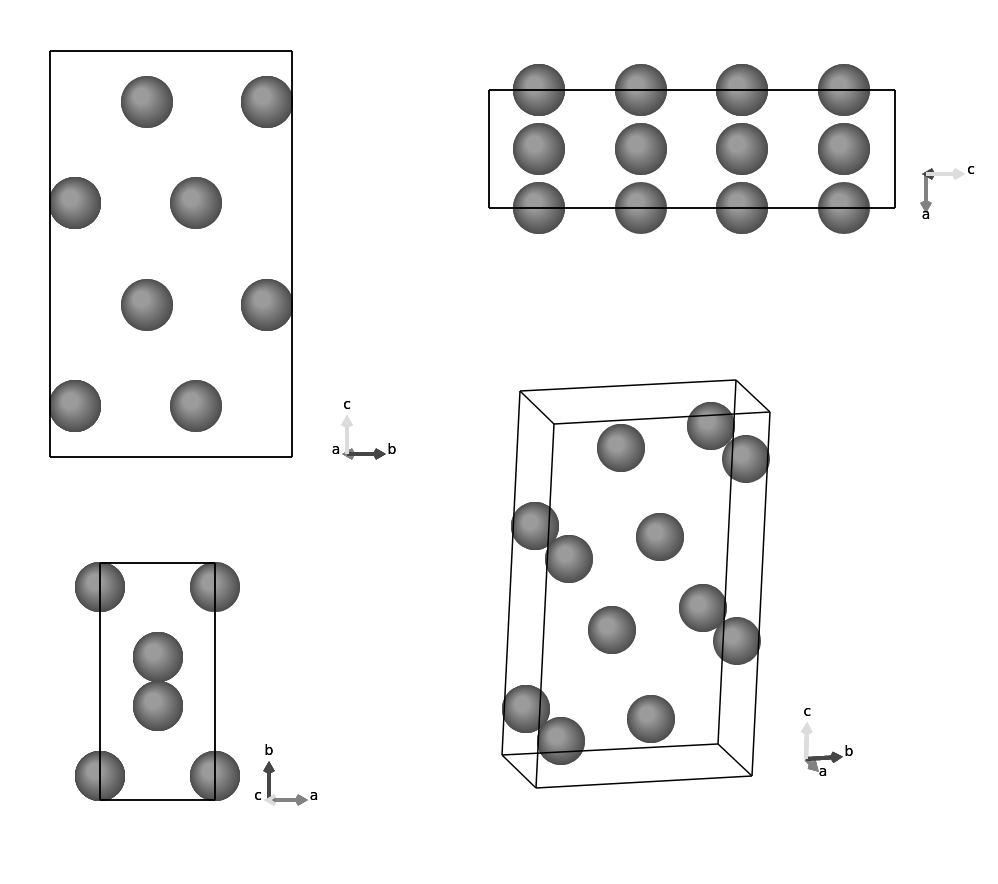
\includegraphics[scale=1.3]{4_image_alphs_greyscale}
\caption{Orthorhombic crystal structure of \textalpha-uranium.}
\label{fig_alphu}
\end{figure}


Alloying uranium to obtain certain properties was extensively studied in the early stages of nuclear fuel development. Some of the reasons were (1) to achieve a finer grain size, (2) to improve mechanical properties, (3) to improve corrosion resistance, and (4) to increase irradiation performance. Aluminum is the material of choice for many components of low-temperature research reactors. The irradiation behavior of aluminum at low temperature ($< 100$\textdegree C) shows favorable behavior, which retains significant ductility and metallic property~\cite{farrell2012}. The uranium--aluminum system has three intermetallic compounds (Fig.~\ref{fig:ualphase}): UAl$_2$, UAl$_3$ and UAl$_4$. UAl$_2$ solidifies at 1615\textdegree C; UAl$_3$ forms at 1355\textdegree C by a peritectic reaction between the solid phase UAl$_2$ and a liquid phase of Al--60wt\%U\@. UAl$_4$ forms at 740\textdegree C by a peritectic reaction between the solid phase UAl$_3$ and a liquid composition of Al--18wt\%U\@. Uranium--aluminum alloys in which the matrix is either primarily aluminum or Al+UAl$_4$ eutectic are widely being used as research reactor fuel. This type of fuel is called a \textit{dispersion}\footnotemark\ fuel.

\footnotetext{A dispersion fuel is one in which the fissile material is contained as a compound dispersed in a nonfissile matrix~\cite{white1957}.}

\begin{figure}
\centering
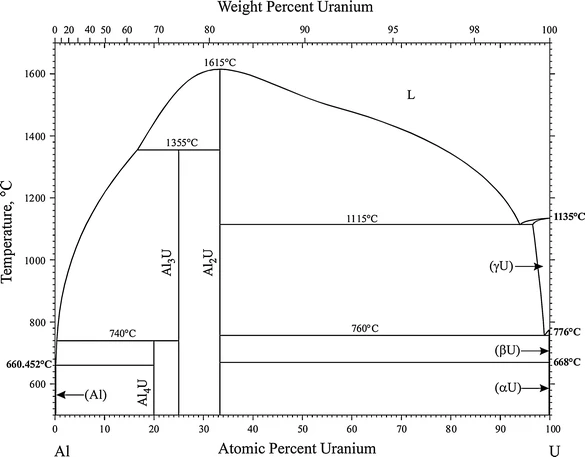
\includegraphics[width=4.75 in]{images/u-al-phase-d.png}
\caption[Uranium--aluminum phase diagram]{Uranium--aluminum phase diagram. Reprinted with permission from Springer Nature: H. Okamoto~\cite{okamoto2012al}, \textcopyright\ 2012\@.}
\label{fig:ualphase}
\end{figure}


Uranium--aluminum alloys can have densities as high as 4.522 gU/cm$^3$~\cite{saller1956study}, but for LEU the required density exceeds 8.5 gU/cm$^3$~\cite{sannen2014}. There are only a few fuel phases with both a high uranium density and stable irradiation properties. The two types of fuels that meet the density requirements are \textgamma-stable uranium and U$_6$Me (Me${}={}$transition metal). U$_6$Me fuels showed very poor irradiation performance at low fission density (\num{3e21} fissions/cm$^3$)~\cite{meyer2000irradiation, hofman1987irradiation, vandenberghe2010}. The \textgamma~phase of uranium can be stabilized by alloying it with suitable elements. Several transition metals stabilize \textgamma-uranium. Elements such as molybdenum (Mo), niobium (Nb), titanium (Ti), and zirconium (Zr) have been tried as alloying elements because of their solubility in \textgamma-uranium~\cite{donze1959stabilisation,giraud1973formation,lopes2013mechanical}. The U--Mo phase diagram (Fig.~\ref{fig:umophase}) has a eutectoid at 11.1 wt\% Mo and 555\textdegree C. If the U--Mo \textgamma~phase contains more than 5 to 7 wt\% Mo, the \textgamma~phase can be retained at room temperature by rapid cooling~\cite{saller1954transformation, bostrom1957}.
 To take advantage of this, uranium alloyed with 10 wt$\%$ molybdenum (U-10Mo) is currently being developed as a potential high-density LEU fuel for high-performance research reactors~\cite{prabhakaran2017u, meyer2014irradiation, williams2017post}. 
%Uranium alloys that retain the high-temperature \textgamma-phase, which is body-centered cubic, are more suitable for reactor fuel due to their more isotropic radiation-induced swelling behavior compared with  \textalpha-uranium~\cite{kittel1993history}.

%The U-Mo alloy has been identified as a high-performance fuel due to its high uranium density and low neutron capture cross-section~\cite{ewh2010microstructural,smirnova2013ternary,rest2009analysis,landa2013density}.



\begin{figure}
\centering

\includegraphics[width=4.75 in]{u-mo-phase-diagram}
\caption[Uranium--molybdenum phase diagram]{Uranium--molybdenum phase diagram\@.\ Reprinted with permission from Springer Nature: H. Okamoto~\cite{okamoto2012mo}, \textcopyright\ 2012\@.}
\label{fig:umophase}
\end{figure}

Before the current interest in U--Mo metallic fuels, some early nuclear reactors used metallic fuels because of the combination of high uranium density and metallic properties. The Godiva IV pulsed reactors at Los Alamos (initially known as \textit{Lady Godiva}) used U--Mo alloys, which date back to 1960~\cite{wimett1965fast}. The Fast Burst Reactor (FBR) at White Sands, the Army Pulsed Radiation Facility (Aberdeen, MD), and the Sandia Pulsed Reactor II also used U--Mo alloys~\cite{wimett1965fast, mihalczo1969static, bonzon1973sandia}. All of these reactors utilized the \textgamma-phase of uranium, but because of their short irradiation time, the impacts of fuel burnup were minimal~\cite{horak1973operating}. Outside USA, the Dounreay Fast Reactor in the U.K. used a number of metal-fuel-based designs, which includes U-9.1Mo (9.1 wt\% Mo) and U-7Mo clad in niobium~\cite{matthews1964performance}. The highly alloyed fuel cracked more, even though the U-9.1Mo fuel swelled slightly less than U-7Mo~\cite{cottrell1964development}. %In U.S. the Enrico Fermi Fast Breeder Reactor (EFFBR) was the first commercial fast reactor that used U--10Mo fuel. 

The primary concern with \textgamma-uranium alloys is to ensure that the fuel remains in the \textgamma~phase during reactor operation. A series of experiments was performed to map the fission rate and temperature dependence of the \textgamma~phase's stability~\cite{no2003iaea}. Two types of U--Mo alloy fuels have been designed and tested. One is monolithic fuel, in which a thin layer of U--Mo foil is bonded to aluminum cladding. The other is a dispersion fuel, in which U--Mo fuel particles are dispersed in an aluminum matrix.



For five decades, dispersion fuels have powered many test and research reactors worldwide. The manufacturing process and operating conditions are well-known for these types of fuels. High-burnup testing of dispersion fuels showed a pattern of \mbox{breakaway} swelling\footnotemark\@ behavior at intermediate burnup. Post-irradiation examinations of U--Mo dispersion fuel revealed that this phenomenon is related to the formation of a ternary aluminide phase. Reaction between the U--Mo fuel kernels and aluminum cladding occurs during irradiation and forms a ternary [(U--Mo)Al$_x$] phase, which releases fission gas at the boundary between the interaction phase and the aluminum matrix~\cite{leenaers2004post,jue2014microstructural,van2008transmission, olander2009growth}. These gas bubbles have a tendency to aggregate into the gas pockets, which weakens the fuel meat by exerting internal pressure. The result is mechanical failure and an increase in fuel volume. To eliminate the fuel--matrix interaction, a `monolithic' U--Mo fuel was suggested. In monolithic fuels, a zirconium foil is used as a diffusion barrier between the fuel and the cladding (aluminum) to prevent diffusion of molybdenum into the cladding~\cite{jue2014microstructural}.

\footnotetext{\textit{Breakaway} is defined as ``the limiting exposure, beyond which there will be a marked increase in the rate of swelling as a function of burnup''~\cite{guay1965}.}



\section{Fission Gas}
The behavior of fission gas---xenon and krypton---has perplexed and fascinated both experimentalists and theorists more than many processes that simultaneously occur in a nuclear fuel elements during irradiation. These inert gases are insoluble in the fuel matrix, causing them to form small gas bubbles. If the gas is released from the fuel, the pressure within the cladding rises, which ultimately results in failure. If the fission gases are retained in the fuel, however, they almost always precipitate as bubbles and cause swelling in the fuel matrix. Swelling adversely impacts the fuel's efficiency. It also impacts the thermal conductivity of the fuel, thereby disrupting the heat extraction from the fuel. One particular xenon isotope, $^{135}$Xe also has a large neutron absorption cross section, which can lead to a reactor ``poisoning.'' As a result, the basic aspects of inert gas behavior are commonly studied for fuel such as UO$_2$.

Xenon is produced directly from fission: 0.3\% of fission products are $^{135}$Xe. It is also produced by the decay of $^{135}$I via the reaction
\begin{equation*}
\ce{^{135}Te ->[$19 \text{s}$] ^{135}I ->[6.7h] ^{135}Xe}.
\end{equation*}
$^{135}$I constitutes almost 6.1\% of fission products. Thus, 95\% of total xenon production is due to the decay of iodine. Xenon is removed from the fuel by  beta decay 
\begin{equation*}
\ce{^{135}Xe ->[9.1 $\text{hr}$] ^{135}Cs + $\beta^{-}$},
\end{equation*}
or by neutron absorption:
\begin{equation*}
\ce{^{135}Xe + ^1_0 n -> ^{136}_{54}Xe + $\gamma$}.
\end{equation*}

In U--Mo fuel, fission gas forms bubbles  both inside the grain and on grain boundaries. Inside the grains, fission gas forms a gas bubble superlattice~\cite{miller2012advantages, gan2010transmission}. 

This dissertation investigates how fission gas (xenon and krypton) impacts the transport properties of U--Mo fuel. Chapter~2 summarizes the theoretical methods used in this work. In Chapter~3, we discuss the reduction of thermal conductivity in U--Mo alloys due to the presence of fission gas. In Chapter~4, we introduce a new pseudopotential for metallic uranium to study its properties using density functional theory (DFT)\@. In Chapter~5, we look into the diffusion mechanism of xenon in \textgamma-uranium and U--Mo alloys. In Chapter~6, we discuss the interaction of helium with a potential plasma-facing material for fusion, lithium, using DFT\@. We discuss conclusions and potential future work in Chapter~7. 


















\bibliographystyle{apsrev4-2}
\bibliography{abbreviated,final}
%\bibliography{abbreviated,firstc}
